\newpage 
\section{A new method for calculating the effect of an induced emotion on a conversation}~\label{sec:approach}
When a user makes an online post, other users can respond to it by liking, sharing, or commenting on it. These actions may elicit additional responses from different users. This results in a conversation graph with reply trees that are rooted in the original post. 
Social media conversation graphs are widely used for a variety of purposes, including sentiment analysis, understanding the various roles users play in a conversation and their influence, predicting the emotion of a response, node prediction, and predicting whether or not a conversation will become toxic, to name a few \cite{yang2022implicit}, \cite{zhao2020modeling}, \cite{yang2017social}, \cite{brambilla2021conversation}. 


Networks from Online Social Networks (OSN) are commonly defined by a graph in which the nodes represent the users in the network and the edges represent the links between the nodes \cite{antonakaki2021survey}. However, in some cases, nodes represent the comments and their responses. In these cases, the nodes in the graph are assigned a weight corresponding to the emotions contained in their text. This weight is then combined with connectivity or centrality-based measures, or it is fed into a Graph Convolutional Network (GCN) to form the prediction. Even though the emotions in the conversation are quantified, they are all treated the same \cite{perikos2018framework}, \cite{albadani2022transformer}. This especially becomes problematic when the nodes in the graphs represent responses/comments instead of users, as the root node now represents the overall emotion of the conversation (as in the previous section of this work). 
 

According to research, outrageous social media expression creates a polarising effect and leads to cluster formation in conversations. Several studies have found that rage-inducing emotions spread faster on social media than positive ones \cite{bacaksizlar2019understanding}, \cite{steinert2022emotions}, \cite{chuai2020anger}, \cite{yi2022depicting}. The amount of rage in a post often determines its virality. This applies to social movements, riots, political posts, and fake news \cite{solovev2022moral}, \cite{mirbabaie2021development}. However, when analysing the emotions in social media posts and performing sentiment analysis to predict the virality or toxicity of an online conversation, this difference in the nature of the diffusion of various emotions is overlooked, and all emotions are weighted equally \cite{yue2019survey}, \cite{nemes2021social}. We believe that taking differences in the nature of emotion diffusion into account will lead to deeper insights into analysing the emotions represented by a post. As a result, we intend to use the empirical analysis of the previous research question, as well as the findings in the literature, to develop a function for assigning weights to the various emotions in a social media conversation. Therefore, in this research we try to answer the following research questions:
\begin{itemize}
    \item How can we quantify the differences in the nature of dispersal and virility of various emotions in social media activities?
    \item What factors define the relationship between the propagation of different emotions on social media and can this relationship be represented by a generalised rule?
    \item How can toxicity be expressed in the form of emotions, or a combination of emotions?
\end{itemize}
\begin{figure}[h]
  
    \centering
    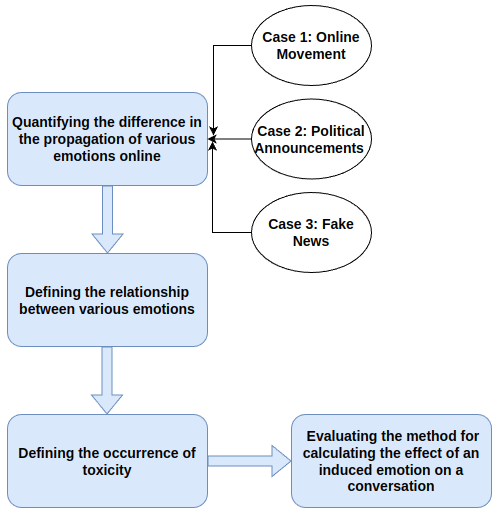
\includegraphics[width=12cm,height=12cm,keepaspectratio]{res2.png}
%   \includegraphics[width=5cm,height=5cm,keepaspectratio]{samples/sample_convv.png}
%   \includegraphics[width=5cm,height=5cm,keepaspectratio]{samples/sample_conv_graphh.png}
  \caption{Proposed methodology for calculating the effect of an induced emotion on a conversation}
  \label{fig:Frameworkres2}
  \end{figure} 
\subsection{Proposed methodology}
\begin{itemize}
    \item The first step involves quantifying the difference in the propagation of various emotions online, by taking into account different cases such as fake news, online movements, political updates etc. as well as considering the various user roles and user engagement on a post. This will help define the relationship between various emotions.
    \item Furthermore, this quantification will be used to define the occurrence of toxicity and whether it is governed by the presence of a single emotion or a certain emotion distribution. To evaluate this function we plan to compare it with the benchmark for toxicity analysis in the literature. This experiment's proposed methodology is shown in Figure-\ref{fig:Frameworkres2}.
\end{itemize}
